\documentclass{book}
\usepackage{graphicx}                              %for PNG images (pdflatex)
\usepackage[linkbordercolor={1.0 1.0 0.0}]{hyperref} %for \url tag
\usepackage{color}                                 %for defining custom colors
\usepackage{framed}                                %for shaded and framed paragraphs
\usepackage{textcomp}                              %for various symbols, e.g. Registered Mark
\usepackage{geometry}                              %for defining page size
\usepackage{longtable}                             %for breaking tables
%
\geometry{verbose,a4paper,tmargin=2.5cm,bmargin=2.5cm,lmargin=2.5cm,rmargin=2cm}
\hypersetup{
  pdfauthor = {Zsombor Nagy},
  pdftitle = {Documentation of the ARC1 storage system},
  pdfsubject = {Paper subject},
  pdfkeywords = {Paper,keyword,comma-separated},
  pdfcreator = {PDFLaTeX with hyperref package},
  pdfproducer = {PDFLaTeX}
}
%
\bibliographystyle{IEEEtran}                       %a nice bibliography style
%
\def\efill{\hfill\nopagebreak}%
\hyphenation{Nordu-Grid}
\setlength{\parindent}{0cm}
\setlength{\FrameRule}{1pt}
\setlength{\FrameSep}{8pt}
\addtolength{\parskip}{5pt}
\renewcommand{\thefootnote}{\fnsymbol{footnote}}
\renewcommand{\arraystretch}{1.3}
\newcommand{\dothis}{\colorbox{shadecolor}}
\newcommand{\globus}{Globus Toolkit\textsuperscript{\textregistered}~2~}
\newcommand{\GT}{Globus Toolkit\textsuperscript{\textregistered}}
\newcommand{\ngdl}{\url{http://ftp.nordugrid.org/download}~}
\definecolor{shadecolor}{rgb}{1,1,0.6}
\definecolor{salmon}{rgb}{1,0.9,1}
\definecolor{bordeaux}{rgb}{0.75,0.,0.}
\definecolor{cyan}{rgb}{0,1,1}
%
%----- DON'T CHANGE HEADER MATTER
\begin{document}
\def\today{\number\day/\number\month/\number\year}

% \begin{titlepage}
% 
% \begin{tabular}{rl}
% \resizebox*{3cm}{!}{
\includegraphics{ng-logo.png}}
% &\parbox[b]{2cm}{\textbf \it {\hspace*{-1.5cm}NORDUGRID\vspace*{0.5cm}}}
% \end{tabular}
% 
% \hrulefill
% 
% %-------- Change this to NORDUGRID-XXXXXXX-NN
% 
% {\raggedleft NORDUGRID-XXXXXXX-NN\par}
% 
% {\raggedleft \today\par}
% 
% \vspace*{2cm}
% 
% %%%%---- The title ----
% {\centering \textsc{\Large Documentation of the ARC1 storage system}\Large \par}
% \vspace*{0.5cm}
%     
% %%%%---- A subtitle, if necessary ----
% {\centering \textit{\large First prototype status and plans}\large \par}
%     
% \vspace*{1.5cm}
% %%%%---- A list of authors ----
%     {\centering \large Zsombor Nagy\footnote{zsombor@niif.hu} \large \par}
%     
% \end{titlepage}
% 
% \tableofcontents                          %Comment if use article style
% \newpage
\chapter{Design Overview}
\label{sec:overview}

% NorduGrid~\cite{nordugrid} Advanced Resource Connector (ARC)
% \textit{middleware}\index{middleware} uses \GT~2 by Globus.
% 
% In expressions, the following operands are allowed:
% \begin{shaded}
%   \verb#=   !=   >   <   >=   <=#
% \end{shaded}
% 
% \begin{framed}
%   Examples of URLs are:\\
%   \\
%   \verb#http://grid.domain.org/dir/script.sh#\\
%   \verb#gsiftp://grid.domain.org:2811;threads=10/dir/input_12378.dat#\\
%   \verb#ldap://grid.domain.org:389/lc=collection1,rc=Nordugrid,dc=nordugrid,dc=org#\\
%   \verb#rc://grid.domain.org/lc=collection1,rc=Nordugrid,dc=nordugrid,dc=org/zebra/f1.zebra#
%   \verb#file:///home/auser/griddir/steer.cra#\\
% \end{framed}

The ARC1 storage system is a distributed system for storing replicated \emph{files} on several file storage nodes and manage them in a global namespace. The files can be grouped into collections, and a \emph{collection} can contain sub-collections and sub-sub-collections in any depth. There is a dedicated \emph{root collection} to gather all collections to the global namespace. This hierarchy of collections and files can be referenced using \emph{Logical Names} (LN). The users can use this global namespace  as they were using a local filesystem. Files can be transfered by multiple transfer protocols, and the client side tools hide this from the user. The replicas of the files are stored on different storage nodes. A storage node should have one or more data transfer service running (e.g. HTTP(S), FTP(S), GridFTP, ByteIO, etc.), and one of the ARC1 storage system’s services is needed to manage each storage node and integrating it into the system. And there are plans to provide a way to integrate third-party storage solutions into the namespace of the ARC1 storage system. The main services are shown on Figure~\ref{fig:services}.

\begin{figure}[ht]
\centering{{\scalebox{0.9}{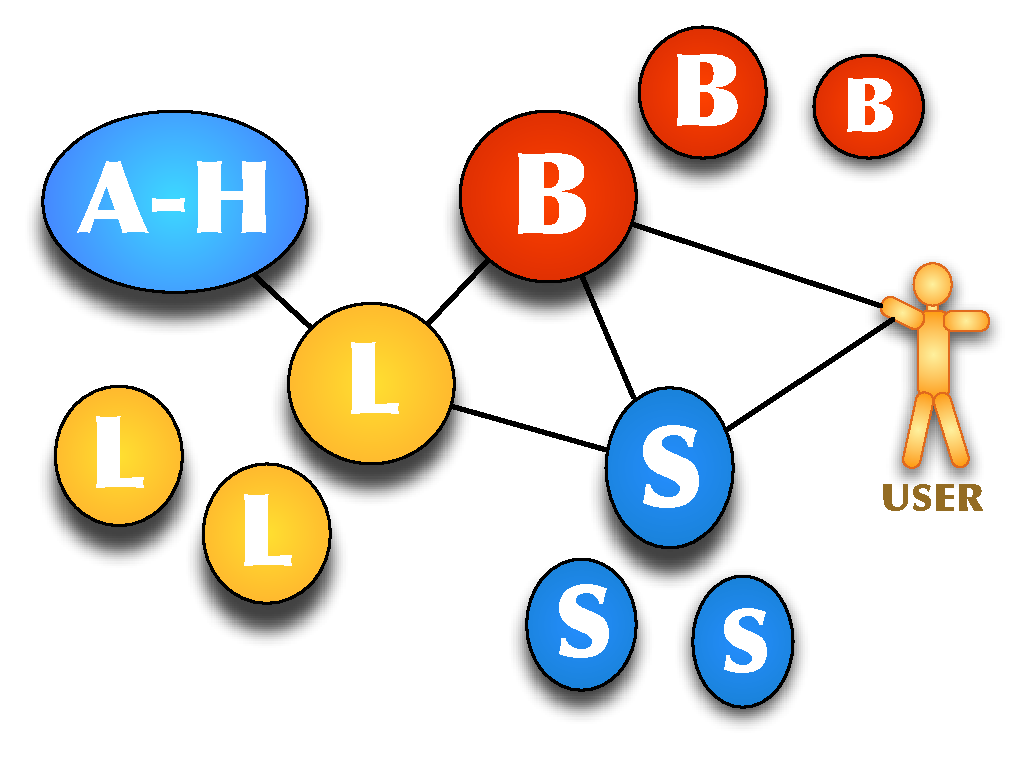
\includegraphics{arc1-storage-services.pdf}}}
\caption{\label{fig:services}The components of the ARC1 storage;
A-H: the \textbf{A-Hash}, which is a currently centralized, later distributed database;
L: the \textbf{Librarian}, which stores the metadata and hierarchy of collections and files, the location of replicas, and health data of the Shepherd services, using the A-Hash as database;
B: the \textbf{Bartender}, which provides a high-level interface for the users and for other services;
S: the \textbf{Shepherd}, which provides a simple interface for storing files on storage nodes.
} }
\end{figure}

\section{IDs used in the system}
\label{sec:IDs}

There are a number of IDs used in the ARC storage system, such as:
\begin{itemize}
    \item Each file and collection has a globally unique ID called \textbf{GUID}.
    \item The files and collections are organized into a global hierarchical namespace and can be referred to using paths of this namespace called \textbf{Logical Names (LN)}.
    \item Each service has a unique \textbf{serviceID} which can be used to get an endpoint reference from the information system. We need an endpoint reference which is an address (URL) which we could connect to.
    \item The Shepherds in the system identify their files using a \textbf{referenceID}.
    \item The \textbf{location} of a replica consists of two IDs: the ID of the Shepherd and the ID of the file within the Shepherd: (serviceID, referenceID).
\end{itemize}

% section IDs (end)

\section{GUIDs and Logical Names (LN)} % (fold)
\label{sec:GUIDsLNs}

The syntax of Logical Names (LN): \verb#/[path]# or \verb#<GUID>[/<path>]# where [...] indicates optional parts.

Each file and collection has a GUID which is globally unique, so they can be unambiguously referred using this GUID, that's why a single GUID is a Logical Name itself.

In a collection each entry has a name, and this entry can be a sub-collection, in which there are files and sub-sub-collections, etc.

\begin{figure}[ht]
\centering{{\scalebox{0.7}{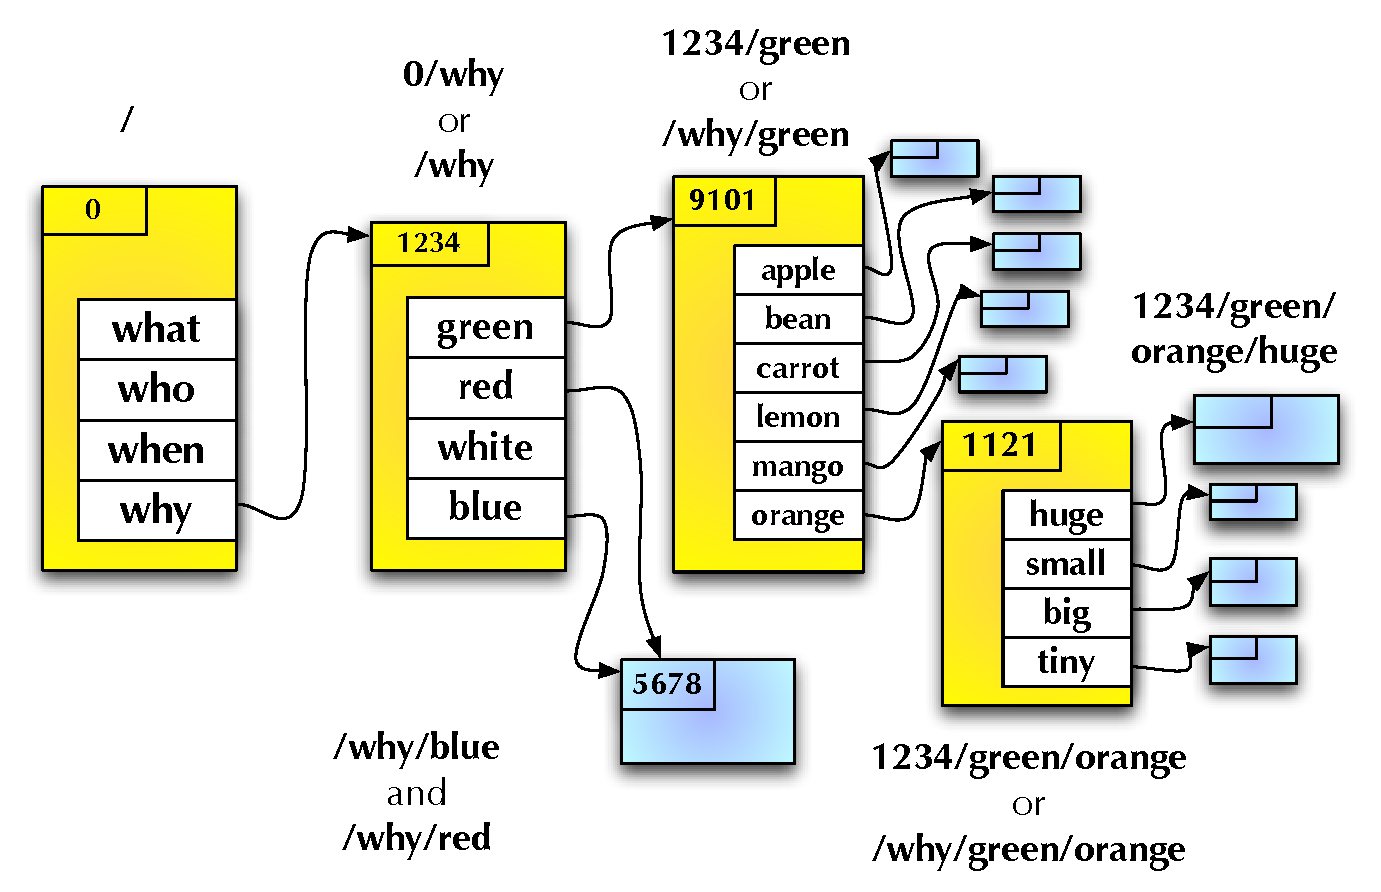
\includegraphics{arc1-storage-namespace.pdf}}}
\caption{\label{fig:namespace}Example of the global namespace's hierarchy} }
\end{figure}

Example on Figure~\ref{fig:namespace}: if we have a collection with GUID \verb#1234#, and there is a collection called \verb#green# in it, and in \verb#green# there is another collection called \verb#orange#, and in \verb#orange# there is a file called \verb#huge#, then we can refer to this file as \verb#/green/orange/huge#, if we know the GUID of the starting collection, so let's prefix the path with it: \verb#1234/green/orange/huge#. This is the Logical Name of that file. If there is a well-known system-wide root collection (its GUID could be e.g. \verb#0#), then if a LN starts with no GUID prefix, it is implicitly prefixed with the GUID of this well-known root collection, e.g. \verb#/why/blue# means \verb#0/why/blue#.

If a client wants to find the file called \verb#/why/blue#, the system knows where to start the search: the GUID of the root collection. The root collection knows the GUID of \verb#why#, and the (sub-)collection \verb#why# knows the GUID of \verb#blue#. If the GUID of this file is \verb#5678#, and somebody makes another entry in collection \verb#/why# (= \verb#0/why#) with name \verb#red# and GUID \verb#5678#, then the \verb#/why/red# LN points to the same file as \verb#/why/blue#, so it's a hard link. To count the references (the number of hardlinks) of a file or collection, the GUID of the parent collection(s) is stored as a metadata for each file and collection.

Each VO should create a VO-wide root collection, and put it in the generic root collection, e.g. if a VO called \verb#vo1# creates a collection called \verb#vo1# as a sub-collection of the root collection (which has the GUID \verb#0#), then it can be referred as \verb#0/vo1# or just \verb#/vo1#. Then this VO can create some files, and put them in this \verb#/vo1# collection, e.g. \verb#/vo1/file1#, etc. Or sub-collections, e.g. \verb#/vo1/col1#, \verb#/vo1/col2/file3#, etc. For this the VO does not need the install any service. These files and collections can be created using a Bartender service.

% section GUIDsLNs (end)

\section{The Bartenders} % (fold)
\label{sec:the_bartenders}
Clients can access the storage system through a Bartender service. If a client wants to create a collection, upload or download a file, the first step is to connect a Bartender. The Bartender then asks a Librarian to resolve Logical Names and return metadata, then initiates file transfers on some storage node by asking the Shepherd service on the node, then returns the transfer URL to the client, which allows the client to directly transfer from/to the storage node. So the data transfer itself is not going through the Bartender, it is performed over a direct link between a storage node and the client.

There could be any number of independent Bartender services in the system which provides high-availability and load-balancing.

% section the_bartenders (end)

\section{The Librarians} % (fold)
\label{sec:the_librarians}
The Librarian is capable of managing the hierarchy and metadata of files and collections, and health information of the Shepherd services. Each file and collection in the Librarian has a globally unique ID (GUID). A collection contains files and other collections, and each of these entries has a name unique within the collection very much like entries in a usual directory on a local filesystem. Besides files and collections the Librarian stores a third type of entries called Mount Points which are references to external services creating the capability to mount the namespace of third-party storages to our global namespace and make the files on a third-party storage available through the interface of the ARC storage system.

The Librarian also manages information about registered Shepherd services which are associated with a storage node, and receives heartbeat messages from them and change replica states automatically if needed.

The Librarian uses the A-Hash as database, that’s why there could be any number of independent Librarian services (all using the same A-Hash) which provides high-availability and load-balancing.

% section the_librarians (end)

\section{The A-Hash} % (fold)
\label{sec:the_a_hash}
The A-Hash is a currently centralized, but later distributed service capable of consistently storing objects containing property-value pairs organized in sections. All metadata about files and collections are stored in the A-Hash, and some information about Shepherd services is stored in it as well.

% section the_a_hash (end)

\section{The Shepherds} % (fold)
\label{sec:the_shepherds}
When a new file is put into the system the number of needed replicas is given for the file. The file replicas are stored on different storage nodes, for each storage node there is Shepherd service which provides the interface for initiating file transfer.

The file-naming used by a Shepherd has nothing to do with the the hierarchy of collections, or Logical Names. When a replica is given to a Shepherd it gets an ID which refers to it within that Shepherd. Each Shepherd has a unique ID itself, so with these IDs the replica can be unambiguously referenced, this is called a Location. The namespace of these Locations has nothing to do with the namespace of GUIDs or the namespace of Logical Names. It consists of two IDs: the ID of the Shepherd and the ID of the file within the Shepherd: \verb!(serviceID, referenceID)!

% section the_shepherds (end)

\section{Heartbeats and replication} % (fold)
\label{sec:heartbeats_and_replication}
Each Shepherd should periodically send heartbeats to a Librarian service with information about replicas whose state changed since the last heartbeat, the Librarian stores these file lists (which contains the GUIDs of the files as well), and if it doesn’t receive a heartbeat for a Shepherd in a given time, it invalidates all the replicas the Shepherd stores. This invalidating means that the state of that location will be \verb!offline!.

If a Shepherd finds out that a file is missing or has a bad checksum, it reports that the file is \verb#invalid# to the Librarian immediately, and the Librarian alters the state of the given replica of the file.

The Shepherd tries to recover its replica by downloading it from another Shepherd. In order to do this the Shepherd contacts a Bartender and asks for the file. The Bartender chooses a valid replica, initiate file transfer by a Shepherd having a valid replica, and returns the TURL to the Shepherd with the invalid replica. The Shepherd with the invalid replica downloads the file from the other Shepherd, and if everything is OK, signals to the Librarian that the replica is \verb!alive! again.

The Shepherds periodically ask the Librarian whether the files they store have enough replicas. If a Shepherd finds that one of the files has not enough replica it turns to a Bartender offering replication. The Bartender chooses a Shepherd, initiates a put request then returns the TURL to the offering Shepherd which could upload the replica. The Shepherd who now has the new replica notifies the Librarian that the file is \verb!alive!. The Librarian sets the state of this new replica.

% section heartbeats_and_replication (end)

\chapter{Use cases} % (fold)
\label{cha:use_cases}

\section{Downloading a file} % (fold)
\label{sec:downloading_a_file}
\begin{figure}[ht]
\centering{{\scalebox{0.7}{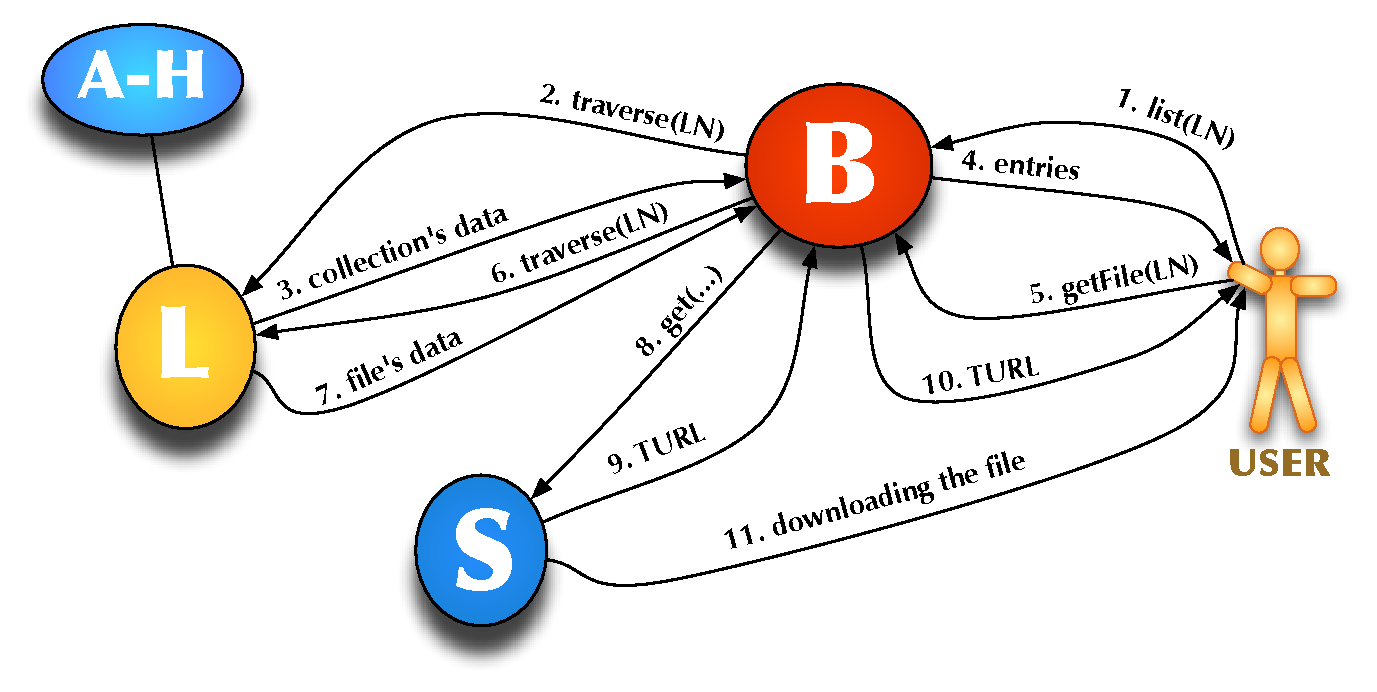
\includegraphics{arc1-storage-downloading.pdf}}}
\caption{\label{fig:downloading}Downloading a file} }
\end{figure}

We want to download a file about which we know that it is somewhere in our home collection on the storage (see Figure~\ref{fig:downloading}). The LN of our home collection is e.g. \verb#/ourvo/users/we#. We can get a list of entries in this collection from any Bartender.

\begin{enumerate}
\item We need to find a Bartender. Maybe we have a cached list of recently used Bartenders or we can get one from the information system. When we have an endpoint reference of a Bartender, we could call its list method with the LN \verb#/ourvo/users/we#.
\item The Bartender has to find a Librarian service, again using its cache of recently used Librarian services or get a new one from the information system. When rhe Bartender has an endpoint reference of a Librarian service, it could ask the Librarian to traverse the LN \verb#/ourvo/users/we#.
\item The Librarian needs the A-Hash service to access the stored data, when it has the endpoint reference of the A-Hash service, it could get the information about the root collection, which contains the GUID of the \verb#ourvo# sub-collection. Then the Librarian gets the entries of this \verb#ourvo# collection, and in it it can find the GUID of \verb#users#, and in the entries of \verb#users# there is the GUID of \verb#we#, which the Librarian returns to the Bartender with all the metadata.
\item The Bartender now has the GUID and the metadata of the collection \verb#/ourvo/users/we#, including the list of its entries. This is returned to us.
\item So we get the list of our \verb#/ourvo/users/we# collection, and now we realize that the file we want has the LN \verb#/ourvo/users/we/thefilewewant# and we know the GUID of it as well: e.g. \verb#a4b2e#. (Of course we know the GUID of the \verb#/ourvo/users/we# collection too, which is e.g. \verb#13245# and using this we could refer to our file as \verb#13245/thefilewewant# which means the entry called \verb#thefilewewant# in the collection with a GUID \verb#13245#.) We connect a Bartender again (the same one or maybe another one) to get the file with any of these LNs, the \verb#a4b2e# is the fastest solution because the Bartender need not to look up the whole LN again in the Librarian, a well-written client API should use this. With the get request we give the Bartender the list of transfer protocols we are able to use.
\item The Bartender contacts the Librarian to get the locations of the replicas of this file.
\item The Librarian returns all the metadata of the requested LN.
\item The Bartender chooses a ‘location’ which consists of the ID of a Shepherd, and the referenceID of the file within the Shepherd. Using the information system or its local cache it could get the endpoint reference of the Shepherd. The Bartender initiates a transfer by the Shepherd, if the Shepherd supports one of the transfer protocols we give, it can create a transfer URL (TURL) with a protocol we can download.
\item The Shepherd returns the TURL to the Bartender.
\item The Bartender returns the TURL to us.
\item Now we have a TURL from which we can download it.
\end{enumerate}

% section downloading_a_file (end)

\section{Uploading a file} % (fold)
\label{sec:uploading_a_file}

\begin{figure}[ht]
\centering{{\scalebox{0.7}{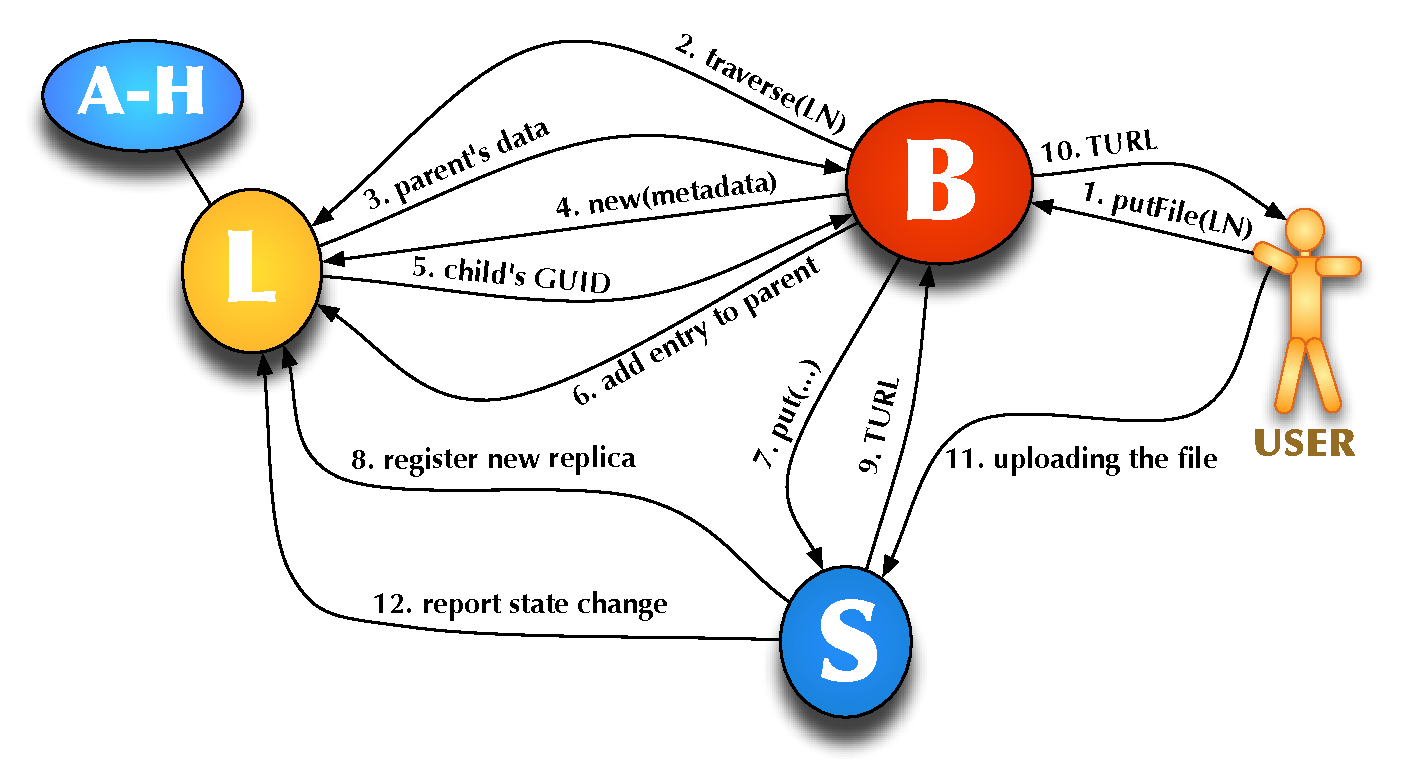
\includegraphics{arc1-storage-uploading.pdf}}}
\caption{\label{fig:uploading}Uploading a file} }
\end{figure}

We have a file on our local disk we want to upload to a collection called \verb#/ourvo/common/docs#. (See Figure~\ref{fig:uploading}.)
\begin{enumerate}
\item We contact a Bartender to put the file, we give the size and checksum and other metadata, and the transfer protocols we want to use. And of course we give the Logical Name we want to be the name of the file, which in this case will be \verb#/ourvo/common/docs/proposal.pdf#
\item The Bartender ask a Librarian to traverse this LN.
\item If the Librarian can traverse the whole LN then this LN is already exists, but if the LN is still available and the parent exists, the Librarian’s response contains the GUID and metadata of the parent collection.
\item Then the Bartender creates a new file entry within the Librarian with all the information we gave. 
\item The Librarian returns the GUID of this new entry.
\item Then the Bartender add the name \verb#proposal.pdf# and the new GUID to the collection \verb#/ourvo/common/docs# and from now on there will be a valid LN \verb#/ourvo/common/docs/proposal.pdf# which points to a file which has no replica at all. If someone tried to download the file called \verb#/ourvo/common/docs/proposal.pdf# now, would get an error message ‘try again later’.
\item The Bartender (using the information system) chooses a Shepherd and gets its endpoint reference. Then the Bartender initiates uploading of the file to the Shepherd: the request includes the size and checksum of the file, the GUID, and the protocols we are able to use.
\item The Shepherd creates a transfer URL and a referenceID for this file and registers the GUID of the file in its own database and reports to the Librarian that there is a new replica with state \verb#creating#. The Librarian gets the message from the Shepherd and creates a new entry in the locations list of the given file with the serviceID and the referenceID the Shepherd have just reported. If someone tries to download this file now, still gets a ‘try again later’ error message, because this new replica is still not \verb#alive#.
\item The Shepherd returns the the TURL to the Bartender.
\item The Bartender returns the TURL to us.
\item Then we can upload the file to this TURL.
\item The Shepherd detects that the file is arrived and reports the change of state to \verb#alive# to the  Librarian who alters the state in the given file-entry. At this point the file has only one replica. 
\end{enumerate}
\begin{itemize}
\item The Shepherd periodically checks the Librarian if this is less than the needed replica number, and if it is then it initiates creating a new replica by a Bartender.
\item The Bartender chooses another Shepherd, initiates the transfer then returns the TURL to the  first Shepherd which uploads the file to the new Shepherd.
\item All the Shepherds check periodically whether their files have enough replica, and if any of them find that there is more replica needed, it initiates creating a new. If more than one Shepperd of course could cause that there will be more replicas than needed. If a Shepherd finds out that a file has more replicas than needed it notifies a Bartender about it.
\item The Bartender ask the Librarian about all Shepherds this file has replicas on, flags this file as ‘removing a replica’ which prevents other Bartenders to remove an other replica accidentally, then make a decision of which one is to be removed, then contacts the chosen Shepherd and asks it to remove the replica. The Shepherd then notify the Librarian, and the Librarian removes the replica, and removes the flag ‘removing a replica’ as well.
\item If we cannot upload the file to the given TURL for some reason, we should remove the file entry from the collection, or we should call \verb#addReplica# to get a new TURL without removing and recreating the file.
\end{itemize}

% section uploading_a_file (end)

\section{Removing a file} % (fold)
\label{sec:removing_a_file}

\begin{figure}[ht]
\centering{{\scalebox{0.7}{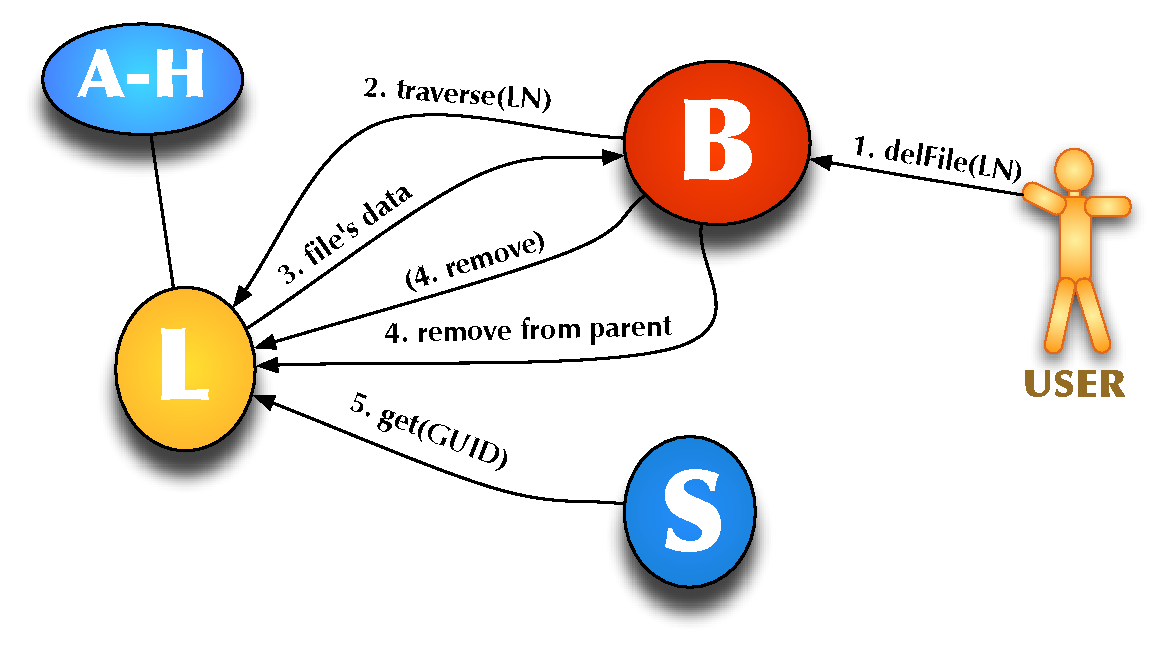
\includegraphics{arc1-storage-removing.pdf}}}
\caption{\label{fig:removing}Removing a file} }
\end{figure}
\begin{enumerate}
    \item If we want to remove a file, we should connect to a Bartender with the LN of the file we want to remove.
    \item The Bartender asks the Librarian to traverse the LN and return the list of parent collections of this file.
    \item The Librarian returns the data.
    \item If the file has only parent, it asks the Librarian to remove the file entry itself, and the entry from the parent collection. If the file has more parent collections (hardlinks) the Bartender only removes the entry from the parent collection and removes the parent from the list of parent  collections of this file.
    \item Next time the Shepherd does its periodic check, it asks the Librarian about each of its stored replicas, and finds out that one of them no longer exists, so it removes the replica from the storage node.
\end{enumerate}


% section removing_a_file (end)

% chapter use_cases (end)

\chapter{Technical description and implementation status} % (fold)
\label{cha:technical_description_and_implementation_status}

The current version of the prototype has no information system and no security, these are soon to be integrated to the system.
The information system is needed to discover services, and to translate serviceIDs to endpoint references (URLs). Currently the URLs are written in the configuration files, and the Shepherd services are reporting their URLs to the Librarian, so the Bartender could ask for all alive Shepherds.

The security is needed to do proper authorization of the users, and to manage access policies of files and collections. ARC has its own policy language, for each file and collection there will be a policy XML document stored as a metadata. The storage services will use the properties extracted from the communication channel and these policies to make authorization decisions. If the properties and the policies are present, the decision is actually made by the security framework of HED.
These are the planned actions which can be used for access control:
\begin{itemize}
    \item \emph{read}: user can get the list of entries in the collection; user can download the file
    \item \emph{addEntry}: user can add a new entry to the collection;
    \item \emph{removeEntry}: user can remove any entry from the collection 
    \item \emph{delete}: user can delete the collection if it is empty; user can delete a file (if you want to remove a file/collection, then the Bartender needs to remove the entry from the parent collection, and then delete the file/collection itself, so you need to have both permissions)
    \item \emph{modifyPolicy}: user can modify the policy of the file/collection
    \item \emph{modifyStates}: user can modify some special metadata of the file/collection (close the collection, change the number of needed replica of the file)
    \item \emph{modifyMetadata}: user can modify the arbitrary metadata section of the file/collection (these are key-value pairs)
\end{itemize}
When a user has the permission in the Librarian to download a file then the user should have permission to access at least one of the file's replica, so there should be a Shepherd which allows the user the get the file. If the Bartender has permission to access the Shepherd, then the Bartender should create an assertion which allows the user to access the file. This could be a signed token which contain a policy defining access to particular file. But all these are currently just plans.

Further prototype statuses and plans can be found below within each section about the services.

% chapter technical_description_and_implementation_status (end)

\section{A-Hash} % (fold)
\label{sec:a_hash}

\subsection{Functionality} % (fold)

The A-Hash is a distributed service capable of storing objects containing property-value pairs grouped in sections in a scalable manner. Each object has an arbitrary string ID, and contains any number of property-value pairs grouped in sections, where property, value and section are arbitrary strings. There could only be one value for a property in a section.

If you have an ID, you can get all property-value pairs of the corresponding object with the \emph{get} method, or you could specify only which sections or properties you need. You can add or remove property-value pairs of an object or delete all occurrences of a property or create a new object with the \emph{change} method, and you can specify conditions, which means the change is only applied if the given conditions are met.

% subsection functionality (end)

\subsection{Prototype status and plans} % (fold)

The A-Hash service currently implemented as a single central service, which stores the data on disk in separate files per object. In the fall of 2008 it will be reimplemented on a distributed hash table (DHT) algorithm, for example the Chord algorithm with a consistency solution called Etna on top of it. This reimplementation hopefully won’t change the interface of the service.

% subsection prototype_status_and_plans (end)

\subsection{Data model} % (fold)

\begin{itemize}
    \item \emph{ID} is an arbitrary string
    \item \emph{object} contains property-value pairs in sections, technically it is a list of key-value pairs where the key is a (section, property) tuple
\end{itemize}

% subsection data_model (end)

\subsection{Interface} % (fold)

\begin{description}
\item [get(ids, neededMetadata)] returns \emph{getResponse} which is a list of (\emph{ID}, \emph{object}) pairs.

The \emph{ids} is a list of string \emph{ID}s, \emph{neededMetadata} is a list of (\emph{section}, \emph{property}) pairs. For each \emph{ID} it returns all the \emph{value}s for each \emph{property} in each \emph{section} (filtered by \emph{neededMetadata}), so \emph{object} is a list of (\emph{section}, \emph{property}, \emph{value}) tuples.

\item [change(changeRequest)] returns \emph{changeResponse} which is a list of (\emph{changeID}, \emph{success}, \emph{failedConditionID}) tuples.

\emph{changeRequest} is a tuple of (\emph{changeID}, \emph{ID}, \emph{changeType}, \emph{section}, \emph{property}, \emph{value}, \emph{conditions}), where \emph{changeID} is an arbitrary ID to identify in the response which change was successful; \emph{ID} points to the object we want to change; \emph{changeType} can be `\textbf{set}' (set the property within the section to value), `\textbf{unset}' (remove the property from the section regardless of the value), `\textbf{delete}' (removes the whole object), conditions is a list of (\emph{conditionID}, \emph{type}, \emph{section}, \emph{property}, \emph{value}) tuples, where \emph{type} could be `\textbf{is}' (the property in the section is set to the value), `\textbf{isnot}' (the property in the section is not set to the value), `\textbf{isset}' (the property of the section is set to any value), `\textbf{unset}' (the property of the section is not set at all).
If all conditions are met, tries to apply changes to the objects, creates a new object if a previously non-existent ID is given. If one of the conditions is not met, returns the ID of the failed condition.
\end{description}
    
% subsection interface (end)

% section a_hash (end)

\section{Librarian} % (fold)
\label{sec:librarian}

\subsection{Functionality} % (fold)
% 
The Librarian manages a tree-hierarchy of files, grouping them into collections. There is a root collection with a well-known GUID which can be used as starting point when resolving Logical Names. If you create a new collection with the method \emph{new}, the Librarian generates a new GUID, but does not insert it into the tree-hierarchy which can be done by adding this GUID as a new entry to one of the existing collection using the \emph{modifyMetadata} method of the existing collection which makes it the parent of the new collection. A collection can be closed via metadata modification which cannot be undone and prevents files to be added or removed from this collection. A new file  also can be created with the \emph{new} method which returns the newly generated GUID of the new file entry which should be added to a parent collection to insert it into the global namespace. A file has a list of locations where its replicas are stored, this list too can be manipulated with \emph{modifyMetadata}. The access policies of the files and collections are also stored as metadata. The \emph{remove} method deletes an entry from the Librarian. The \emph{traverseLN} method try to traverse Logical Names by walking the hierarchy of the namespace and to return the GUID of the entry pointed by the LN. After you have a GUID of file, collection or mount point, you can get all the information using the \emph{get} method. 

% subsection functionality (end)

\subsection{Prototype status and plans} % (fold)

The Librarian service currently implements all the methods below, but doesn’t do very much error checking. This should be changed, the Librarian should check the validity of metadata, and forbid some cases, e.g. reopen a closed collection.

% subsection prototype_status_and_plans (end)

\subsection{Data model} % (fold)
\label{sub:data_model}
Each librarian entry has a unique ID called \emph{GUID}.

The Librarian uses the A-Hash to store all the data about the files and collections. The A-Hash is capable of storing property-value pairs organized in sections, which actually means that it stores (\emph{section}, \emph{property}, \emph{value}) tuples where each member is simply a string, e.g. (‘entry’, ’type’, ’collection’) or (‘ACL’, ’johnsmith’, ’owner’) or (‘timestamps’, ’created’, ’1196265901’) or (‘locations’, ’64CDF45F-DDFA-4C1D-8D08-BCF7810CB2AB:9A293F27DC86’, ’sentenced’). There could be only one value for a (\emph{section}, \emph{property}) pair.

\begin{itemize}
    \item A \textbf{collection} is a list of files and other collections, which are in parent-children relationships forming a tree-hierarchy. Each entry has a name which is only valid within this collection, and it is unique within the collection. Each entry is referenced by its GUID. So the metadata sections of a collection are as follows: 
    \begin{description}
        \item [entry] section 
        \begin{itemize}
            \item \emph{type}: `collection' 
        \end{itemize}
        \item [entries] section 
        \begin{itemize}
            \item \emph{(name, GUID) pairs}: a Collection is basically a list of name-GUID pairs. 
        \end{itemize}
        \item [timestamps] section 
        \begin{itemize}
            \item \emph{created}: timestamp of creation 
            \item \emph{modified}: timestamp of last modification 
        \end{itemize}
        \item [states] section 
        \begin{itemize}
            \item closed: if the collection is closed, then nothing can be added to its contents 
        \end{itemize}
        \item [policies] section 
        \begin{itemize}
            \item XML representations of access policies 
        \end{itemize}
        \item [metadata] section 
        \begin{itemize}
            \item any other arbitrary metadata 
        \end{itemize}
    \end{description}
    \item A \textbf{file} entry contains the following sections: 
    \begin{description}
        \item [entry] section 
        \begin{itemize}
            \item \emph{type}: `file' 
        \end{itemize}
        \item [locations] section 
        \begin{itemize}
            \item \emph{(location, state) pairs}, where a location is a (\emph{serviceID}, \emph{referenceID}) pair serialized as a  string, where \emph{serviceID} is the ID of the Shepherd service storing this replica, \emph{referenceID} is the ID of the file within that Shepherd service, and state could be `\textbf{alive}' (if the replica passed the checksum test, and the storage element storing it is healthy), `\textbf{invalid}' (if the replica has wrong checksum, or the storage element claims it has no such file), `\textbf{offline}' (if the storage element is not reachable, but may have a valid replica), `\textbf{creating}' (if the replica is in the state of uploading), `\textbf{sentenced}' (if the replica is marked for deletion) 
        \end{itemize}
        \item [timestamps] section 
        \begin{itemize}
            \item \emph{created}: timestamp of creation 
            \item \emph{modified}: timestamp of last modification (e.g. modification of metadata)
        \end{itemize}
        \item [states] section 
        \begin{itemize}
            \item \emph{size}: the file size in bytes
            \item \emph{checksum}: checksum of the file
            \item \emph{checksumType}: the name of the checksum method
            \item \emph{neededReplicas}: how many valid replicas should this file have 
        \end{itemize}
        \item [policies] section 
        \begin{itemize}
            \item XML representations of access policies 
        \end{itemize}
        \item [metadata] section 
        \begin{itemize}
            \item any other arbitrary metadata 
        \end{itemize}
    \end{description}
    \item There is one more type of Librarian entries called \textbf{mount point} which is a reference to a service which is capable of handling a subtree of the namespace. The properties of a mount point in sections:
    \begin{description}
        \item [entry] section 
        \begin{itemize}
            \item \emph{type}: `mountpoint' 
        \end{itemize}
        \item [mount] section 
        \begin{itemize}
            \item \emph{target}: the ID of the service
            \item \emph{ID}: an ID within the service (optional)
        \end{itemize}
        \item [timestamps] section 
        \begin{itemize}
            \item \emph{created}: timestamp of creation 
            \item \emph{modified}: timestamp of last modification (e.g. modification of metadata)
        \end{itemize}
        \item [policies] section 
        \begin{itemize}
            \item XML representations of access policies 
        \end{itemize}
        \item [metadata] section 
        \begin{itemize}
            \item any other arbitrary metadata 
        \end{itemize}
    \end{description}

    \item The Librarian stores information about the Shepherds, so each Shepherd has a GUID as well. There is an entry (with GUID `1’ by default) which contains the GUID and the timestamp of the last heartbeat for each registered Shepherd:
    \begin{description}
    	\item [nextHeartBeat] section
    	\begin{itemize}
    		\item (ID, timestamp) pairs
    	\end{itemize}
    	\item [serviceGUID] section
        \begin{itemize}
            \item (ID, GUID) pairs
        \end{itemize}
    \end{description}

    \item For each Shepherd there is a separate entry with the list of files:
    \begin{description}
    	\item [entry] section
        \begin{itemize}
            \item \emph{type}: `shepherd'
        \end{itemize}
    	\item [file] section
    	\begin{itemize}
    	    \item \emph{(referenceID, GUID) pairs} for each replica stored on the Shepherd
    	\end{itemize}
    \end{description}
\end{itemize}

% subsection data_model (end)

% section librarian (end)

\bibliography{grid}
\end{document}
